\chapter{Scintillator detector}
\label{ch:detector}


\section{Signal performance of a detector}
\label{sec:detector-signal}

\subsection{Scintillator uniformity}

Monte Carlo simulation of signal transport in the detector predicts a non-uniform signal transmission for particles passing through different positions of the detector. This is experimentally confirmed by coincidence tests using a \SI[product-units = repeat]{1 x 1}{\centi\meter} scintillator connected to a \pmt and the standard detector. The small detector was then placed on various location on top of the large detector. Particles passing through both detectors are selected using a coincidence trigger. This way the position of the particle in the large detector is known and the efficiency at specific points can be determined. In \cref{fig:scintilator_transmission_compared} the results from the experiment and the simulation for the various positions are compared.

\begin{figure}
    \centering
    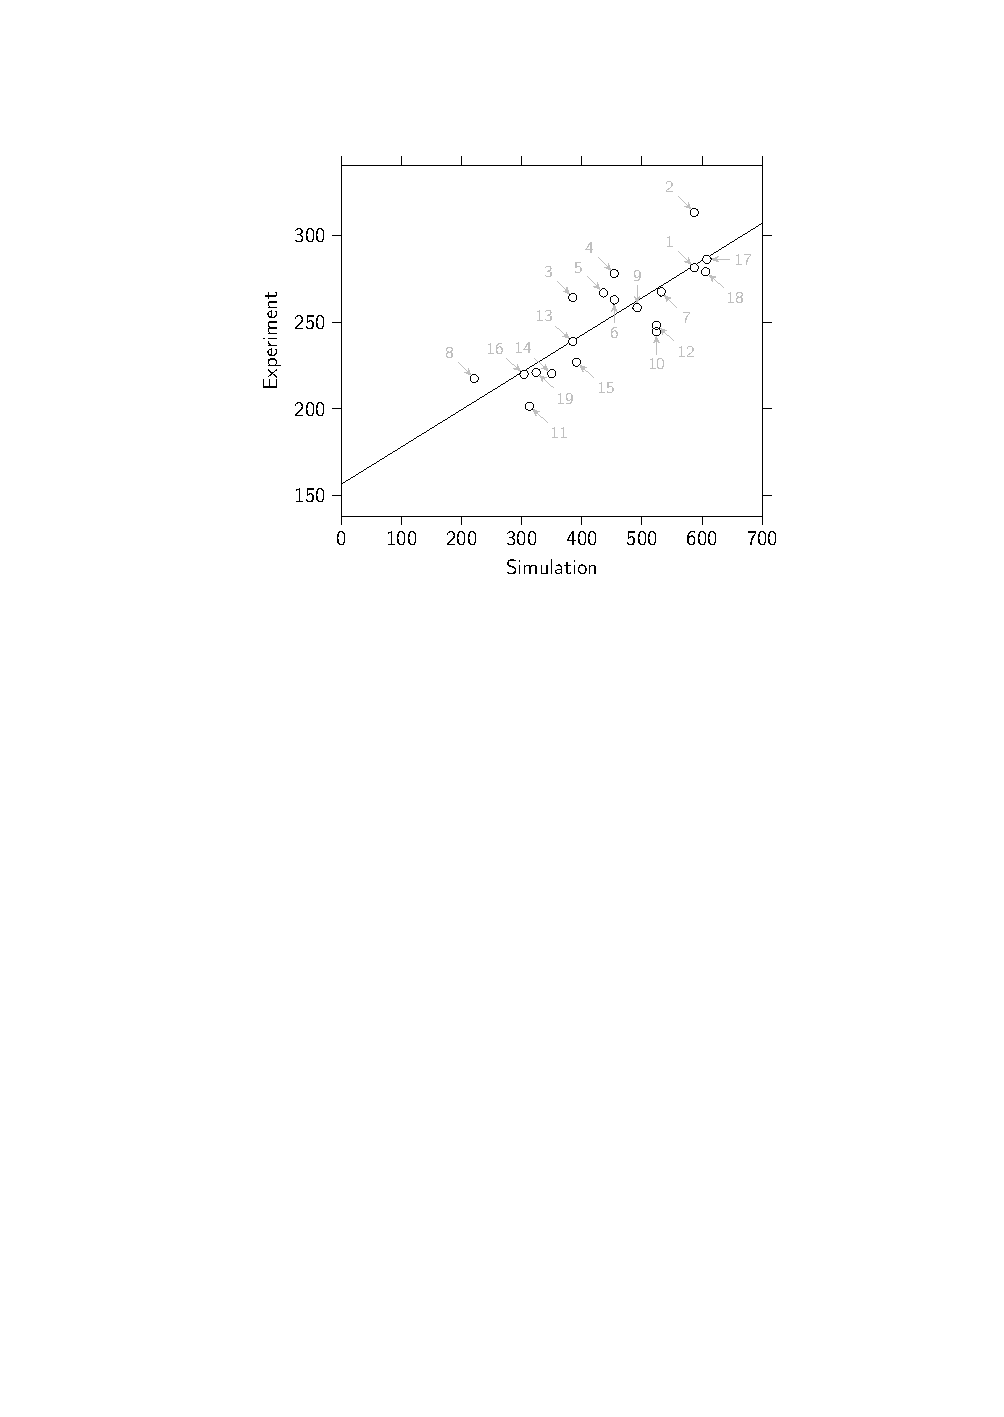
\includegraphics{plots/detector/scintilator_transmission_compared}
    \caption{Correlation between the transmission efficiency for different positions in the scintillator between a real HiSPARC detector and the simulated one. The difference can be explained by the aluminium foil in which the detector is wrapped is not taken into account in the simulation. Moreover, some of the positions are in locations where the simulation predicts a significant gradient.}
    \label{fig:scintilator_transmission_compared}
\end{figure}

In the detector simulation the distribution in \cref{fig:signal_efficiency} is used to simulate the signal strength caused by each particle in a detector. First combining the Bethe-Bloch formula and energy-straggling results in the Landau distribution, for vertical particles. The Landau distribution gives the amount of energy lost by particles which pass through the detector. In the simulations the exact location in the detector is ignored. Therefore, the Landau distribution is convolved with the transmission efficiency distribution of the detectors. The resulting distribution can be scaled by $\cos{\theta}^{-1}$ for particles arriving at angles in the detector.

\begin{figure}
    \centering
    % \usepackage{tikz}
% \usetikzlibrary{arrows}
% \usepackage{pgfplots}
% \pgfplotsset{compat=1.3}
% \usepackage[detect-family]{siunitx}
% \usepackage[eulergreek]{sansmath}
% \sisetup{text-sf=\sansmath}
% \usepackage{relsize}
%
\tikzsetnextfilename{externalized-signal_efficiency}
\pgfkeysifdefined{/artist/width}
    {\pgfkeysgetvalue{/artist/width}{\defaultwidth}}
    {\def\defaultwidth{ .67\linewidth }}
%
%
\begin{sansmath}
\begin{tikzpicture}[
        font=\sffamily,
        every pin/.style={inner sep=2pt, font={\sffamily\smaller}},
        every label/.style={inner sep=2pt, font={\sffamily\smaller}},
        every pin edge/.style={<-, >=stealth', shorten <=2pt},
        pin distance=2.5ex,
    ]
    \begin{axis}[
            axis background/.style={  },
            xmode=normal,
            ymode=normal,
            width=\defaultwidth,
            axis equal=false,
            %
            title={  },
            %
            xlabel={ Signal strength [\si{\mip}] },
            ylabel={ Counts },
            %
            xmin={  },
            xmax={  },
            ymin={ 0.0 },
            ymax={  },
            %
            xtick={  },
            ytick={  },
            %
            tick align=outside,
            max space between ticks=40,
            every tick/.style={},
            axis on top,
        ]

        






    
    % Draw series plot
    \addplot[no markers,solid,const plot] coordinates {
        (0.0, 0)
        (0.05, 0)
        (0.1, 0)
        (0.15, 0)
        (0.2, 0)
        (0.25, 0)
        (0.3, 0)
        (0.35, 0)
        (0.4, 0)
        (0.45, 5)
        (0.5, 62)
        (0.55, 121)
        (0.6, 205)
        (0.65, 277)
        (0.7, 349)
        (0.75, 397)
        (0.8, 476)
        (0.85, 563)
        (0.9, 604)
        (0.95, 676)
        (1.0, 635)
        (1.05, 681)
        (1.1, 582)
        (1.15, 549)
        (1.2, 505)
        (1.25, 471)
        (1.3, 411)
        (1.35, 365)
        (1.4, 344)
        (1.45, 292)
        (1.5, 235)
        (1.55, 184)
        (1.6, 152)
        (1.65, 145)
        (1.7, 112)
        (1.75, 122)
        (1.8, 103)
        (1.85, 83)
        (1.9, 86)
        (1.95, 58)
        (2.0, 47)
        (2.05, 43)
        (2.1, 32)
        (2.15, 17)
        (2.2, 10)
        (2.25, 1)
        (2.3, 0)
        (2.35, 0)
        (2.4, 0)
        (2.45, 0)
    };







    \end{axis}
\end{tikzpicture}
\end{sansmath}

    \caption{Signal distribution for one particle. This distribution gives the signal from a single particles passing straight through a random location of the scintillator. The distribution scales with $\cos{\theta}^{-1}$.}
    \label{fig:signal_efficiency}
\end{figure}


\subsection{\pmt linearity}

In an EAS many more than one particle may pass through a detector. The response of the \pmt to different signal sizes needs to be investigated to determine the accuracy with which the number of particles can be reconstructed. Ideally the output of the \pmt grows linearly with the number of photons impacting its photocathode. Large signals from the \pmt, capable of saturating the \adc, are expected to occur dozens of times a day. However, in the data we find that some \pmts never produce signals that saturate the \adc. Calibration tests have been performed on several \pmts to test their output given a known input signal.


\subsection{PMT calibration}
\label{sub:pmt_calibration}

A setup has been created to test the linearity of \pmts using LED light flashes. A bundle of 24 optical fibers, each connected to a LED, are fed into a cap which directs the light at the window of a \pmt. The LEDs can be triggered simultaneously to produce a short (\SI{20}{\ns}) pulse. This is similar to a pulse generator, but with light. The intensity of light produced on the \pmt by a single fiber is comparable to one or two \mip in a detector. The pulse-to-pulse intensity typically fluctuates by \SI{50}{\percent}. Taking the average over hundreds of pulses gives a very stable result.

\begin{figure}
    \centering
    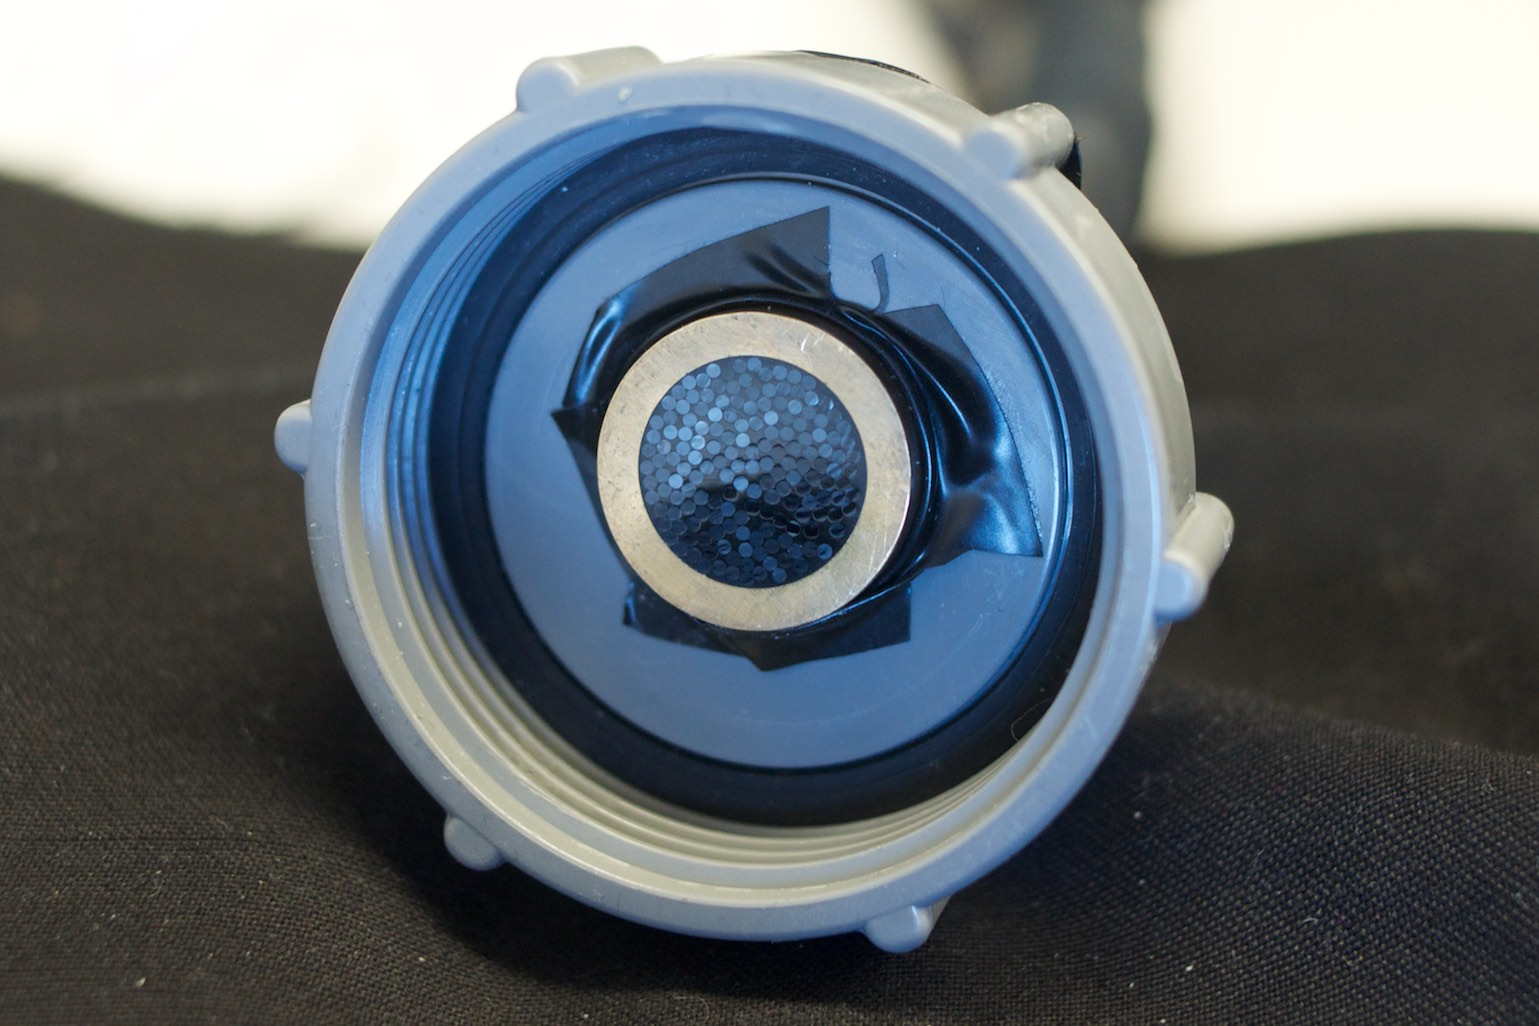
\includegraphics[width=.45\linewidth]{plots/detector/ARN_085351.jpg}
    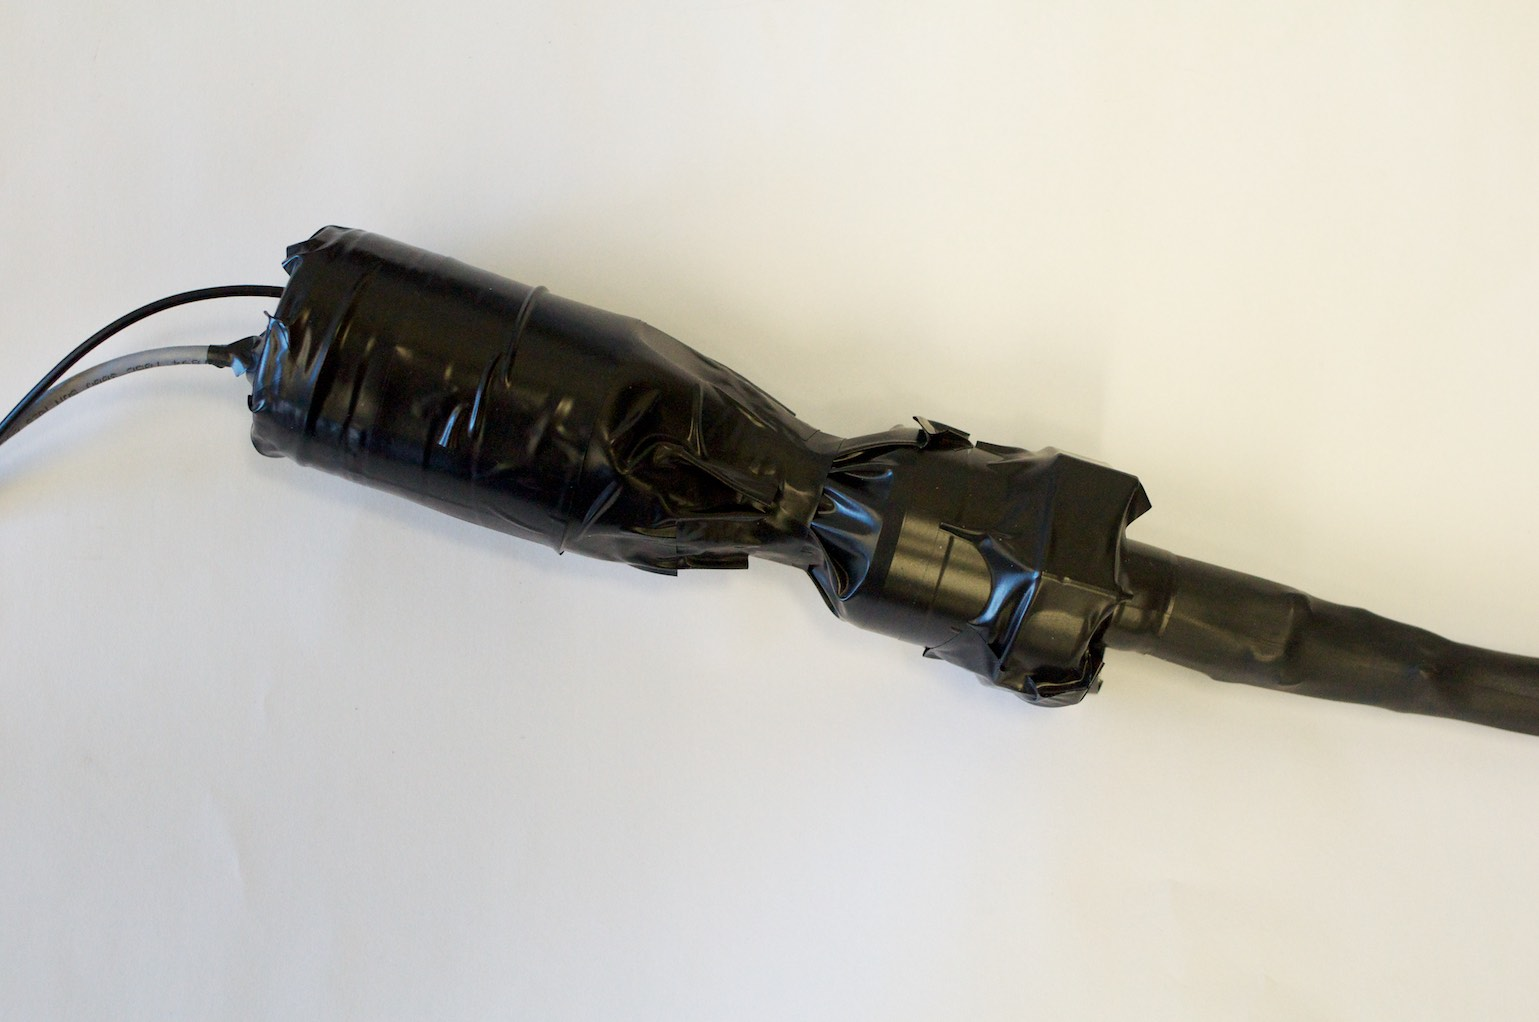
\includegraphics[width=.45\linewidth]{plots/detector/ARN_085349.jpg}
    \caption{Here the setup for the PMT tests is shown. The first photo shows the fibers in the bundle. The second photo shows the bundle connected to the \pmt, wrapped light tight with tape.}
    \label{fig:pmt_test_setup}
\end{figure}

The mean intensity of the individual fibers is not equal. For each \pmt the mean intensity of each individual fiber is determined. This is done by disconnecting and darkening the other fibers. This makes it possible to determine the input signal when multiple fibers are connected. This is expected to be the sum of the individual signals. Possible time delays between the pulses might make the resulting pulses wider instead of higher, so not only the pulse height is examined but also the pulse integral. Any subset of the 24 fibers can be used simultaneously. Signals with and expected \pmt output pulse over \SI{5}{\volt} are possible with the full bundle of fibers, with the \pmt is still at normal operating voltage.

An oscilloscope is used to readout the \pmt signal. This allows for easy averaging of multiple signals and to readout signals larger than \SI{2}{\volt}. The oscilloscope measures the signal's pulse height and integral.

In \cref{fig:linearity_pmts} the results of two \pmt tests are shown. The \senstech \pmt already start to be non-linear before the pulse height reaches \SI{1}{\volt}. With increased signal input it just barely reaches \SI{2}{\volt}. The \nikhef \pmt on the other hand is linear over the entire range that was measured. The tests confirm that the \nikhef produced \pmt power supplies can supply enough current to saturate the \hisparc electronics. Larger input signals were not possible with the used setup, so it remains unclear at what point it will be unable to keep up. The non-linear curve can be fitted by the following equation, as described in \cite{icecube2010pmt}.

\begin{equation}
    \ln V_{\mathrm{in}} = \ln V +
                          \frac{p_0 \left(\frac{V}{p_1}\right)^{p_2}}
                               {\left(1 - \frac{V}{p_1}\right)^{\frac{1}{4}}}
\end{equation}

Where $V$ is the measured output signal and $V_{in}$ the input. The parameters ($p_{1,2,3}$) have no physical meaning.

\begin{figure}
    \centering
    % \usepackage{tikz}
% \usetikzlibrary{arrows,external}
% \usepackage{pgfplots}
% \pgfplotsset{compat=1.3}
% \usepackage[detect-family]{siunitx}
% \usepackage[eulergreek]{sansmath}
% \sisetup{text-sf=\sansmath}
% \usepackage{relsize}
%
    \tikzsetnextfilename{externalized-linearity_compared}
\pgfkeysifdefined{/artist/width}
    {\pgfkeysgetvalue{/artist/width}{\defaultwidth}}
    {\def\defaultwidth{ .6\linewidth }}
%
    \pgfkeysifdefined{/artist/height}
        {\pgfkeysgetvalue{/artist/height}{\defaultheight}}
        {\def\defaultheight{ .6\linewidth }}
%
\begin{sansmath}
\begin{tikzpicture}[
        font=\sffamily,
        every pin/.style={inner sep=2pt, font={\sffamily\smaller}},
        every label/.style={inner sep=2pt, font={\sffamily\smaller}},
        every pin edge/.style={<-, >=stealth', shorten <=2pt},
        pin distance=2.5ex,
    ]
    \begin{axis}[
            axis background/.style={  },
            xmode=normal,
            ymode=normal,
            width=\defaultwidth,
                height=\defaultheight,
            scale only axis,
            axis equal=true,
            %
            title={  },
            %
            xlabel={ Sum individual LED pulse heights [V] },
            ylabel={ Multiple-LED pulse height [V] },
            %
            xmin={ 0 },
            xmax={ 6005 },
            ymin={ 0 },
            ymax={ 6005 },
            %
            xtick={ 0, 1000, 2000, 3000, 4000, 5000, 6000 },
            ytick={ 0, 1000, 2000, 3000, 4000, 5000, 6000 },
            xticklabels={  0, 1, 2, 3, 4, 5, 6 },
            yticklabels={  0, 1, 2, 3, 4, 5, 6 },
            xticklabel style={  },
            yticklabel style={  },
            %
            tick align=outside,
            max space between ticks=40,
            every tick/.style={},
            axis on top,
            point meta min={  },
            point meta max={  },
                colormap={coolwarm}{
                    rgb255(0cm)=( 59, 76,192);
                    rgb255(1cm)=( 98,130,234);
                    rgb255(2cm)=(141,176,254);
                    rgb255(3cm)=(184,208,249);
                    rgb255(4cm)=(221,221,221);
                    rgb255(5cm)=(245,196,173);
                    rgb255(6cm)=(244,154,123);
                    rgb255(7cm)=(222, 96, 77);
                    rgb255(8cm)=(180,  4, 38)},
        ]





    % Draw series plot
    \addplot[mark=*,mark options=white,only marks] coordinates {
            (5050, 5050)
            (4671, 4723)
            (4379, 4396)
            (3953, 3950)
            (3466, 3560)
            (3030, 3150)
            (2600, 2686)
            (2075, 2140)
            (1685, 1746)
            (1194, 1224)
            (722, 716)
            (348, 318)
    };


    % Draw series plot
    \addplot[mark=*,only marks] coordinates {
            (412, 325)
            (572, 550)
            (754, 730)
            (934, 860)
            (1130, 1000)
            (1289, 1120)
            (1529, 1267)
            (1719, 1339)
            (1959, 1453)
            (2203, 1545)
            (2405, 1605)
            (2655, 1712)
            (2875, 1776)
            (3077, 1844)
            (3240, 1877)
            (3539, 1960)
            (3721, 1983)
            (3951, 2036)
            (4406, 2097)
            (4782, 2150)
            (4932, 2170)
    };


    % Draw series plot
    \addplot[mark=o,only marks] coordinates {
            (5050, 5050)
            (4671, 4723)
            (4379, 4396)
            (3953, 3950)
            (3466, 3560)
            (3030, 3150)
            (2600, 2686)
            (2075, 2140)
            (1685, 1746)
            (1194, 1224)
            (722, 716)
            (348, 318)
    };


    % Draw series plot
    \addplot[no markers,solid] coordinates {
            (326.895910995, 325.0)
            (330.671772439, 328.69739479)
            (334.449956614, 332.394789579)
            (338.230505781, 336.092184369)
            (342.013462519, 339.789579158)
            (345.798869719, 343.486973948)
            (349.586770591, 347.184368737)
            (353.377208656, 350.881763527)
            (357.170227752, 354.579158317)
            (360.965872032, 358.276553106)
            (364.764185963, 361.973947896)
            (368.565214329, 365.671342685)
            (372.369002228, 369.368737475)
            (376.175595075, 373.066132265)
            (379.9850386, 376.763527054)
            (383.797378851, 380.460921844)
            (387.61266219, 384.158316633)
            (391.430935297, 387.855711423)
            (395.252245171, 391.553106212)
            (399.076639126, 395.250501002)
            (402.904164795, 398.947895792)
            (406.73487013, 402.645290581)
            (410.568803402, 406.342685371)
            (414.4060132, 410.04008016)
            (418.246548434, 413.73747495)
            (422.090458336, 417.434869739)
            (425.937792457, 421.132264529)
            (429.78860067, 424.829659319)
            (433.642933171, 428.527054108)
            (437.50084048, 432.224448898)
            (441.362373439, 435.921843687)
            (445.227583214, 439.619238477)
            (449.096521299, 443.316633267)
            (452.969239511, 447.014028056)
            (456.845789996, 450.711422846)
            (460.726225227, 454.408817635)
            (464.610598004, 458.106212425)
            (468.498961457, 461.803607214)
            (472.391369049, 465.501002004)
            (476.28787457, 469.198396794)
            (480.188532145, 472.895791583)
            (484.09339623, 476.593186373)
            (488.002521618, 480.290581162)
            (491.915963433, 483.987975952)
            (495.83377714, 487.685370741)
            (499.756018537, 491.382765531)
            (503.682743763, 495.080160321)
            (507.614009296, 498.77755511)
            (511.549871954, 502.4749499)
            (515.490388898, 506.172344689)
            (519.435617631, 509.869739479)
            (523.385616, 513.567134269)
            (527.340442201, 517.264529058)
            (531.300154772, 520.961923848)
            (535.264812602, 524.659318637)
            (539.23447493, 528.356713427)
            (543.209201345, 532.054108216)
            (547.189051788, 535.751503006)
            (551.174086554, 539.448897796)
            (555.164366293, 543.146292585)
            (559.159952012, 546.843687375)
            (563.160905078, 550.541082164)
            (567.167287213, 554.238476954)
            (571.179160505, 557.935871743)
            (575.196587403, 561.633266533)
            (579.219630719, 565.330661323)
            (583.248353633, 569.028056112)
            (587.282819692, 572.725450902)
            (591.323092812, 576.422845691)
            (595.36923728, 580.120240481)
            (599.421317758, 583.817635271)
            (603.479399279, 587.51503006)
            (607.543547255, 591.21242485)
            (611.613827476, 594.909819639)
            (615.69030611, 598.607214429)
            (619.773049708, 602.304609218)
            (623.862125206, 606.002004008)
            (627.957599924, 609.699398798)
            (632.059541571, 613.396793587)
            (636.168018243, 617.094188377)
            (640.283098432, 620.791583166)
            (644.404851018, 624.488977956)
            (648.533345283, 628.186372745)
            (652.6686509, 631.883767535)
            (656.810837948, 635.581162325)
            (660.959976904, 639.278557114)
            (665.116138651, 642.975951904)
            (669.279394478, 646.673346693)
            (673.449816082, 650.370741483)
            (677.62747557, 654.068136273)
            (681.812445466, 657.765531062)
            (686.004798705, 661.462925852)
            (690.204608641, 665.160320641)
            (694.41194905, 668.857715431)
            (698.626894129, 672.55511022)
            (702.849518499, 676.25250501)
            (707.07989721, 679.9498998)
            (711.318105741, 683.647294589)
            (715.564220004, 687.344689379)
            (719.818316345, 691.042084168)
            (724.080471548, 694.739478958)
            (728.350762838, 698.436873747)
            (732.62926788, 702.134268537)
            (736.916064787, 705.831663327)
            (741.211232119, 709.529058116)
            (745.514848887, 713.226452906)
            (749.826994555, 716.923847695)
            (754.147749043, 720.621242485)
            (758.477192732, 724.318637275)
            (762.815406463, 728.016032064)
            (767.162471543, 731.713426854)
            (771.518469744, 735.410821643)
            (775.883483314, 739.108216433)
            (780.257594969, 742.805611222)
            (784.640887905, 746.503006012)
            (789.033445797, 750.200400802)
            (793.435352802, 753.897795591)
            (797.846693563, 757.595190381)
            (802.267553212, 761.29258517)
            (806.698017375, 764.98997996)
            (811.138172169, 768.687374749)
            (815.588104215, 772.384769539)
            (820.047900631, 776.082164329)
            (824.517649044, 779.779559118)
            (828.997437586, 783.476953908)
            (833.487354903, 787.174348697)
            (837.987490155, 790.871743487)
            (842.497933023, 794.569138277)
            (847.018773707, 798.266533066)
            (851.550102935, 801.963927856)
            (856.092011963, 805.661322645)
            (860.644592581, 809.358717435)
            (865.207937113, 813.056112224)
            (869.782138426, 816.753507014)
            (874.367289928, 820.450901804)
            (878.963485578, 824.148296593)
            (883.570819882, 827.845691383)
            (888.189387904, 831.543086172)
            (892.819285266, 835.240480962)
            (897.460608153, 838.937875752)
            (902.113453317, 842.635270541)
            (906.777918079, 846.332665331)
            (911.454100337, 850.03006012)
            (916.142098565, 853.72745491)
            (920.842011823, 857.424849699)
            (925.553939756, 861.122244489)
            (930.277982599, 864.819639279)
            (935.014241184, 868.517034068)
            (939.762816942, 872.214428858)
            (944.523811908, 875.911823647)
            (949.297328724, 879.609218437)
            (954.083470645, 883.306613226)
            (958.882341544, 887.004008016)
            (963.694045912, 890.701402806)
            (968.518688871, 894.398797595)
            (973.356376168, 898.096192385)
            (978.207214187, 901.793587174)
            (983.071309954, 905.490981964)
            (987.948771134, 909.188376754)
            (992.839706044, 912.885771543)
            (997.744223656, 916.583166333)
            (1002.6624336, 920.280561122)
            (1007.59444616, 923.977955912)
            (1012.5403723, 927.675350701)
            (1017.50032366, 931.372745491)
            (1022.47441254, 935.070140281)
            (1027.46275195, 938.76753507)
            (1032.46545555, 942.46492986)
            (1037.48263773, 946.162324649)
            (1042.51441357, 949.859719439)
            (1047.56089883, 953.557114228)
            (1052.62221001, 957.254509018)
            (1057.6984643, 960.951903808)
            (1062.78977964, 964.649298597)
            (1067.89627465, 968.346693387)
            (1073.01806873, 972.044088176)
            (1078.15528198, 975.741482966)
            (1083.30803525, 979.438877756)
            (1088.47645015, 983.136272545)
            (1093.66064902, 986.833667335)
            (1098.86075499, 990.531062124)
            (1104.07689194, 994.228456914)
            (1109.30918449, 997.925851703)
            (1114.55775809, 1001.62324649)
            (1119.82273894, 1005.32064128)
            (1125.10425402, 1009.01803607)
            (1130.40243113, 1012.71543086)
            (1135.71739886, 1016.41282565)
            (1141.0492866, 1020.11022044)
            (1146.39822456, 1023.80761523)
            (1151.76434376, 1027.50501002)
            (1157.14777605, 1031.20240481)
            (1162.54865413, 1034.8997996)
            (1167.9671115, 1038.59719439)
            (1173.40328255, 1042.29458918)
            (1178.85730247, 1045.99198397)
            (1184.32930735, 1049.68937876)
            (1189.81943414, 1053.38677355)
            (1195.32782063, 1057.08416834)
            (1200.85460552, 1060.78156313)
            (1206.39992839, 1064.47895792)
            (1211.9639297, 1068.17635271)
            (1217.54675081, 1071.87374749)
            (1223.14853401, 1075.57114228)
            (1228.76942247, 1079.26853707)
            (1234.40956029, 1082.96593186)
            (1240.06909252, 1086.66332665)
            (1245.74816513, 1090.36072144)
            (1251.44692501, 1094.05811623)
            (1257.16552004, 1097.75551102)
            (1262.90409903, 1101.45290581)
            (1268.66281177, 1105.1503006)
            (1274.44180901, 1108.84769539)
            (1280.2412425, 1112.54509018)
            (1286.06126495, 1116.24248497)
            (1291.90203009, 1119.93987976)
            (1297.76369265, 1123.63727455)
            (1303.64640837, 1127.33466934)
            (1309.550334, 1131.03206413)
            (1315.47562734, 1134.72945892)
            (1321.42244721, 1138.42685371)
            (1327.39095348, 1142.1242485)
            (1333.38130708, 1145.82164329)
            (1339.39366999, 1149.51903808)
            (1345.42820527, 1153.21643287)
            (1351.48507707, 1156.91382766)
            (1357.5644506, 1160.61122244)
            (1363.66649219, 1164.30861723)
            (1369.79136927, 1168.00601202)
            (1375.93925039, 1171.70340681)
            (1382.11030521, 1175.4008016)
            (1388.30470453, 1179.09819639)
            (1394.52262029, 1182.79559118)
            (1400.76422561, 1186.49298597)
            (1407.02969472, 1190.19038076)
            (1413.31920307, 1193.88777555)
            (1419.63292725, 1197.58517034)
            (1425.97104507, 1201.28256513)
            (1432.33373553, 1204.97995992)
            (1438.72117883, 1208.67735471)
            (1445.13355639, 1212.3747495)
            (1451.57105089, 1216.07214429)
            (1458.03384621, 1219.76953908)
            (1464.5221275, 1223.46693387)
            (1471.03608117, 1227.16432866)
            (1477.5758949, 1230.86172345)
            (1484.14175764, 1234.55911824)
            (1490.73385965, 1238.25651303)
            (1497.35239247, 1241.95390782)
            (1503.99754898, 1245.65130261)
            (1510.66952337, 1249.34869739)
            (1517.36851116, 1253.04609218)
            (1524.09470922, 1256.74348697)
            (1530.84831578, 1260.44088176)
            (1537.62953045, 1264.13827655)
            (1544.4385542, 1267.83567134)
            (1551.27558941, 1271.53306613)
            (1558.14083984, 1275.23046092)
            (1565.03451068, 1278.92785571)
            (1571.95680856, 1282.6252505)
            (1578.90794153, 1286.32264529)
            (1585.88811909, 1290.02004008)
            (1592.89755222, 1293.71743487)
            (1599.93645335, 1297.41482966)
            (1607.00503643, 1301.11222445)
            (1614.10351688, 1304.80961924)
            (1621.23211166, 1308.50701403)
            (1628.39103923, 1312.20440882)
            (1635.58051961, 1315.90180361)
            (1642.80077437, 1319.5991984)
            (1650.05202662, 1323.29659319)
            (1657.33450107, 1326.99398798)
            (1664.64842404, 1330.69138277)
            (1671.9940234, 1334.38877756)
            (1679.3715287, 1338.08617234)
            (1686.78117108, 1341.78356713)
            (1694.22318335, 1345.48096192)
            (1701.69779996, 1349.17835671)
            (1709.20525704, 1352.8757515)
            (1716.74579244, 1356.57314629)
            (1724.31964566, 1360.27054108)
            (1731.92705796, 1363.96793587)
            (1739.56827231, 1367.66533066)
            (1747.24353344, 1371.36272545)
            (1754.95308784, 1375.06012024)
            (1762.69718377, 1378.75751503)
            (1770.47607128, 1382.45490982)
            (1778.29000224, 1386.15230461)
            (1786.13923034, 1389.8496994)
            (1794.02401111, 1393.54709419)
            (1801.94460193, 1397.24448898)
            (1809.90126205, 1400.94188377)
            (1817.89425261, 1404.63927856)
            (1825.92383665, 1408.33667335)
            (1833.99027915, 1412.03406814)
            (1842.093847, 1415.73146293)
            (1850.23480905, 1419.42885772)
            (1858.41343613, 1423.12625251)
            (1866.63000105, 1426.82364729)
            (1874.88477862, 1430.52104208)
            (1883.17804569, 1434.21843687)
            (1891.51008112, 1437.91583166)
            (1899.88116585, 1441.61322645)
            (1908.2915829, 1445.31062124)
            (1916.74161736, 1449.00801603)
            (1925.23155644, 1452.70541082)
            (1933.7616895, 1456.40280561)
            (1942.33230802, 1460.1002004)
            (1950.94370566, 1463.79759519)
            (1959.59617827, 1467.49498998)
            (1968.2900239, 1471.19238477)
            (1977.02554283, 1474.88977956)
            (1985.80303757, 1478.58717435)
            (1994.62281291, 1482.28456914)
            (2003.48517592, 1485.98196393)
            (2012.39043597, 1489.67935872)
            (2021.33890475, 1493.37675351)
            (2030.33089631, 1497.0741483)
            (2039.36672705, 1500.77154309)
            (2048.44671577, 1504.46893788)
            (2057.57118366, 1508.16633267)
            (2066.74045436, 1511.86372745)
            (2075.95485393, 1515.56112224)
            (2085.21471094, 1519.25851703)
            (2094.52035643, 1522.95591182)
            (2103.87212395, 1526.65330661)
            (2113.2703496, 1530.3507014)
            (2122.71537205, 1534.04809619)
            (2132.20753254, 1537.74549098)
            (2141.74717491, 1541.44288577)
            (2151.33464564, 1545.14028056)
            (2160.97029387, 1548.83767535)
            (2170.6544714, 1552.53507014)
            (2180.38753275, 1556.23246493)
            (2190.16983514, 1559.92985972)
            (2200.00173856, 1563.62725451)
            (2209.88360577, 1567.3246493)
            (2219.81580233, 1571.02204409)
            (2229.79869661, 1574.71943888)
            (2239.83265985, 1578.41683367)
            (2249.91806614, 1582.11422846)
            (2260.0552925, 1585.81162325)
            (2270.24471885, 1589.50901804)
            (2280.48672808, 1593.20641283)
            (2290.78170605, 1596.90380762)
            (2301.13004164, 1600.6012024)
            (2311.53212674, 1604.29859719)
            (2321.98835633, 1607.99599198)
            (2332.49912846, 1611.69338677)
            (2343.06484429, 1615.39078156)
            (2353.68590815, 1619.08817635)
            (2364.36272753, 1622.78557114)
            (2375.09571312, 1626.48296593)
            (2385.88527884, 1630.18036072)
            (2396.73184188, 1633.87775551)
            (2407.63582271, 1637.5751503)
            (2418.59764513, 1641.27254509)
            (2429.61773628, 1644.96993988)
            (2440.6965267, 1648.66733467)
            (2451.83445032, 1652.36472946)
            (2463.03194452, 1656.06212425)
            (2474.28945017, 1659.75951904)
            (2485.60741163, 1663.45691383)
            (2496.98627679, 1667.15430862)
            (2508.42649715, 1670.85170341)
            (2519.92852776, 1674.5490982)
            (2531.49282736, 1678.24649299)
            (2543.11985833, 1681.94388778)
            (2554.81008675, 1685.64128257)
            (2566.56398246, 1689.33867735)
            (2578.38201906, 1693.03607214)
            (2590.26467395, 1696.73346693)
            (2602.21242839, 1700.43086172)
            (2614.22576751, 1704.12825651)
            (2626.30518036, 1707.8256513)
            (2638.45115992, 1711.52304609)
            (2650.66420319, 1715.22044088)
            (2662.94481116, 1718.91783567)
            (2675.2934889, 1722.61523046)
            (2687.71074559, 1726.31262525)
            (2700.19709451, 1730.01002004)
            (2712.75305315, 1733.70741483)
            (2725.37914321, 1737.40480962)
            (2738.07589063, 1741.10220441)
            (2750.84382565, 1744.7995992)
            (2763.68348284, 1748.49699399)
            (2776.59540115, 1752.19438878)
            (2789.58012395, 1755.89178357)
            (2802.63819904, 1759.58917836)
            (2815.77017876, 1763.28657315)
            (2828.97661994, 1766.98396794)
            (2842.25808404, 1770.68136273)
            (2855.61513712, 1774.37875752)
            (2869.04834991, 1778.0761523)
            (2882.55829786, 1781.77354709)
            (2896.14556117, 1785.47094188)
            (2909.81072484, 1789.16833667)
            (2923.55437874, 1792.86573146)
            (2937.37711762, 1796.56312625)
            (2951.27954115, 1800.26052104)
            (2965.26225401, 1803.95791583)
            (2979.32586591, 1807.65531062)
            (2993.47099163, 1811.35270541)
            (3007.6982511, 1815.0501002)
            (3022.00826941, 1818.74749499)
            (3036.40167688, 1822.44488978)
            (3050.87910911, 1826.14228457)
            (3065.44120703, 1829.83967936)
            (3080.08861695, 1833.53707415)
            (3094.82199059, 1837.23446894)
            (3109.64198517, 1840.93186373)
            (3124.54926344, 1844.62925852)
            (3139.54449373, 1848.32665331)
            (3154.62835002, 1852.0240481)
            (3169.80151197, 1855.72144289)
            (3185.06466499, 1859.41883768)
            (3200.41850031, 1863.11623246)
            (3215.86371501, 1866.81362725)
            (3231.40101206, 1870.51102204)
            (3247.03110044, 1874.20841683)
            (3262.75469515, 1877.90581162)
            (3278.57251725, 1881.60320641)
            (3294.48529399, 1885.3006012)
            (3310.49375878, 1888.99799599)
            (3326.59865133, 1892.69539078)
            (3342.80071767, 1896.39278557)
            (3359.1007102, 1900.09018036)
            (3375.49938779, 1903.78757515)
            (3391.99751581, 1907.48496994)
            (3408.5958662, 1911.18236473)
            (3425.29521755, 1914.87975952)
            (3442.09635515, 1918.57715431)
            (3459.00007105, 1922.2745491)
            (3476.00716415, 1925.97194389)
            (3493.11844023, 1929.66933868)
            (3510.33471207, 1933.36673347)
            (3527.65679944, 1937.06412826)
            (3545.08552926, 1940.76152305)
            (3562.6217356, 1944.45891784)
            (3580.26625978, 1948.15631263)
            (3598.01995042, 1951.85370741)
            (3615.88366357, 1955.5511022)
            (3633.85826268, 1959.24849699)
            (3651.94461879, 1962.94589178)
            (3670.14361051, 1966.64328657)
            (3688.45612415, 1970.34068136)
            (3706.88305375, 1974.03807615)
            (3725.42530123, 1977.73547094)
            (3744.08377639, 1981.43286573)
            (3762.85939702, 1985.13026052)
            (3781.75308898, 1988.82765531)
            (3800.76578628, 1992.5250501)
            (3819.89843117, 1996.22244489)
            (3839.1519742, 1999.91983968)
            (3858.52737431, 2003.61723447)
            (3878.02559892, 2007.31462926)
            (3897.64762401, 2011.01202405)
            (3917.3944342, 2014.70941884)
            (3937.26702285, 2018.40681363)
            (3957.26639214, 2022.10420842)
            (3977.39355315, 2025.80160321)
            (3997.64952596, 2029.498998)
            (4018.03533972, 2033.19639279)
            (4038.55203278, 2036.89378758)
            (4059.20065274, 2040.59118236)
            (4079.98225657, 2044.28857715)
            (4100.89791069, 2047.98597194)
            (4121.94869107, 2051.68336673)
            (4143.13568334, 2055.38076152)
            (4164.45998284, 2059.07815631)
            (4185.92269478, 2062.7755511)
            (4207.52493429, 2066.47294589)
            (4229.26782656, 2070.17034068)
            (4251.15250691, 2073.86773547)
            (4273.1801209, 2077.56513026)
            (4295.35182443, 2081.26252505)
            (4317.66878388, 2084.95991984)
            (4340.13217616, 2088.65731463)
            (4362.74318886, 2092.35470942)
            (4385.50302033, 2096.05210421)
            (4408.41287982, 2099.749499)
            (4431.47398756, 2103.44689379)
            (4454.68757487, 2107.14428858)
            (4478.05488433, 2110.84168337)
            (4501.57716982, 2114.53907816)
            (4525.25569667, 2118.23647295)
            (4549.09174178, 2121.93386774)
            (4573.08659374, 2125.63126253)
            (4597.24155293, 2129.32865731)
            (4621.55793166, 2133.0260521)
            (4646.03705428, 2136.72344689)
            (4670.68025732, 2140.42084168)
            (4695.48888959, 2144.11823647)
            (4720.46431233, 2147.81563126)
            (4745.60789933, 2151.51302605)
            (4770.92103704, 2155.21042084)
            (4796.40512474, 2158.90781563)
            (4822.06157464, 2162.60521042)
            (4847.89181203, 2166.30260521)
            (4873.89727539, 2170.0)
    };


    % Draw series plot
    \addplot[no markers,gray] coordinates {
            (0, 0)
            (6000, 6000)
    };

    \node[,
          below right=2pt
        ]
        at (rel axis cs:0,1)
        { $\mathrm{ln}V_{\mathrm{in}}=\mathrm{ln}V + \frac{p_0\left(\frac{V}{p_1}\right)^{p_2}}{\left(1-\frac{V}{p_1}\right)^{\frac{1}{4}}}$, \scriptsize{($p_0=29.1$, $p_1=9000$, $p_2=2.6$)} };

    \end{axis}
\end{tikzpicture}
\end{sansmath}

    \caption{Measurements of the pulse height linearity of \pmts. The dependence of the pulse height output on the input light intensity is shown. The input on the horizontal axis is in arbitrary units. The data points show the results from tests with the \senstech \pmt (closed circles) and the \nikhef \pmt (open circles). The black line are fits to the data.}
    \label{fig:linearity_pmts}
\end{figure}

The pulse height and pulse integral were both measured during the tests. The relation between these quantities is shown in \cref{fig:ph_pi_compared_nikhef_senstech} for the different \pmts. The relationship is also linear for the \nikhef \pmt, and non-linear for the others.

\begin{figure}
    \centering
    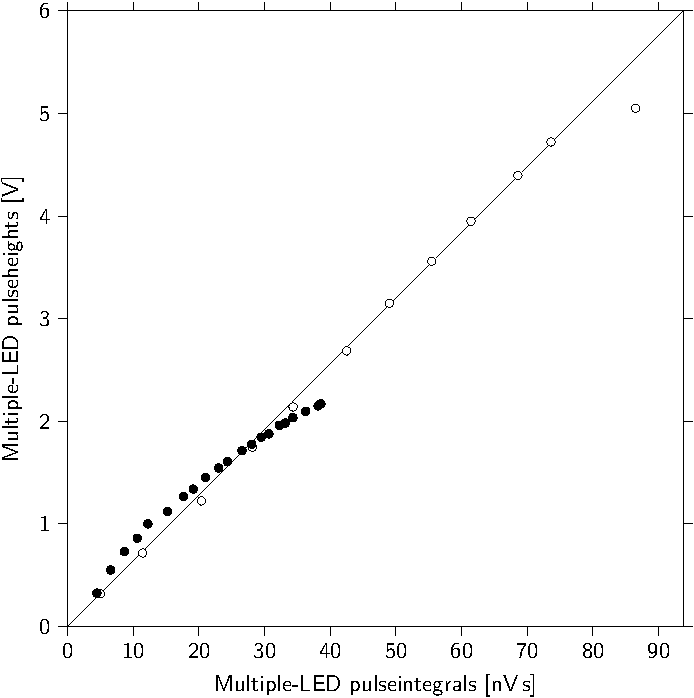
\includegraphics[width=.7\linewidth]
                    {plots/detector/ph_pi_compared_nikhef_senstech}
    \caption{Measurements of the pulse height versus pulse integral. The data points show the results for the \senstech \pmt (closed circles) and the \nikhef \pmt (open circles). The last data point for the \nikhef \pmt has an unexplained offset, possibly due to a bad measurement.}
    \label{fig:ph_pi_compared_nikhef_senstech}
\end{figure}

In \cref{fig:ph_pi_503} cosmic-ray data is shown comparing a \nikhef and \senstech \pmt used in a single station. The \senstech \pmt clearly does not saturate the \adcs, while the other does. The pulse integral does continue to grow for the \nikhef \pmt while its pulse height is saturated. This is explained by the pulse becoming wider at its base. The pulse integral grows slower when some of the samples in the pulse are saturated. The difference seen in this relation for the types of \pmts can be used to identify the \pmt.

\begin{figure}
    \centering
    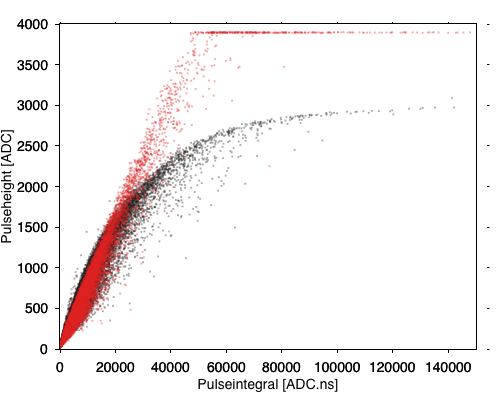
\includegraphics[width=.7\textwidth]{plots/detector/ph_pi_503.png}
    \caption{Measured pulse height versus pulse integral from real detector data. The data is from detector 1 and 2 from station 503. Detector 1 (black) uses a \senstech \pmt, detector 2 (red) uses a \nikhef \pmt.}
    \label{fig:ph_pi_503}
\end{figure}

As can be seen in both the test and cosmic data, the \senstech \pmt is a bit steeper at low pulse integrals. This means that the pulses are less wide. [different number of dynodes?, different voltage?]

For each \senstech \pmt a different correction needs to be applied to the detected signals. Unfortunately, almost no \pmts have been calibrated using the LED setup. Measured cosmic data does provide some insight into the non linearity, however, the pulse height and integral are not independent measurements.

The \adcs in the \hisparc electronics are designed and calibrated to make the range \SIrange{200}{4096}{\adc} correspond to the range \SIrange{0}{-2}{\volt}. Signals greater than \SI{-2}{\volt} are clipped, preventing the pulse height to provide an accurate measure of signal strength. The pulse height clipping also affects the pulse integral. For larger signals the non-saturated parts of the signal also grow bigger, so the integral continues to increase.

In determining the particle density at a detector there are two components to look at. Given a particle density the number of particles that actually pass through a detector follows from the Poisson distribution. The width of the distribution is the square root of the mean value. This means that the error becomes larger for higher densities. Given a number of particles passing through the detector the detected signal size

- List contributions to uncertainty in particle density; Poisson, gamma's, scintillator position, pmt linearity.
- Give total uncertainty on particle density (as function of density).

Since April 2014 new \pmts are first tested in the LED setup using a single fiber to ensure it works properly. The test finds the voltage at which the output has a pulse height around \SI{340}{\milli\volt}. This pulse height value requires a voltage close to the normal operational voltage of \pmts on a \hisparc detector. The current of the \pmt is checked, high currents can indicate failing \pmts.


\section{Environmental conditions}
\label{sec:detector-environmental}

\subsection{Temperature in skibox}

The specifications of the scintillator and \pmt indicate that their efficiency depends on their temperature. The pulse height of signals determine wether they cross the thresholds in the electronics and cause a trigger. The efficiency of the detector may drop such that some events no longer cause a trigger, which they would have under normal circumstances. The change in efficiency also affects the MPV. The amount of effect the temperature has on the MPV will be examined.

About 20 \hisparc stations also have a weather station which includes a temperature sensor recording the outside temperature. The locations of the weather stations are shown in \cref{fig:weather-map}. Such enviornmental data is also available for other locations in the Netherlands from the Dutch Royal Meteorological Institute (KNMI) which operates many weather stations across the Netherlands. However, these are not at the same location as \hisparc stations. For short periods temperature probes have been placed inside the skibox, and attached to the \pmt, of some detectors to accurately measure the temperature of the detector. In \cref{fig:temperature_timeline} the values from these sensors for a month can be seen. The daily (night/day) fluctuations can clearly be seen. The skibox and \pmt temperatures clearly rise above the outside temperature. This is mostly due to the absorption of solar radiation by the skibox, and the heat generated by the \pmt. There is little to no air flow inside the skibox. On sunny days the temperatures in the skibox rise a lot higher than the outside temperature. Using solar radiation data the outside temperature can be corrected to accurately describe the skibox temperature (see \cite{devries2012weather} fig 7.7).

\begin{figure}
    \centering
    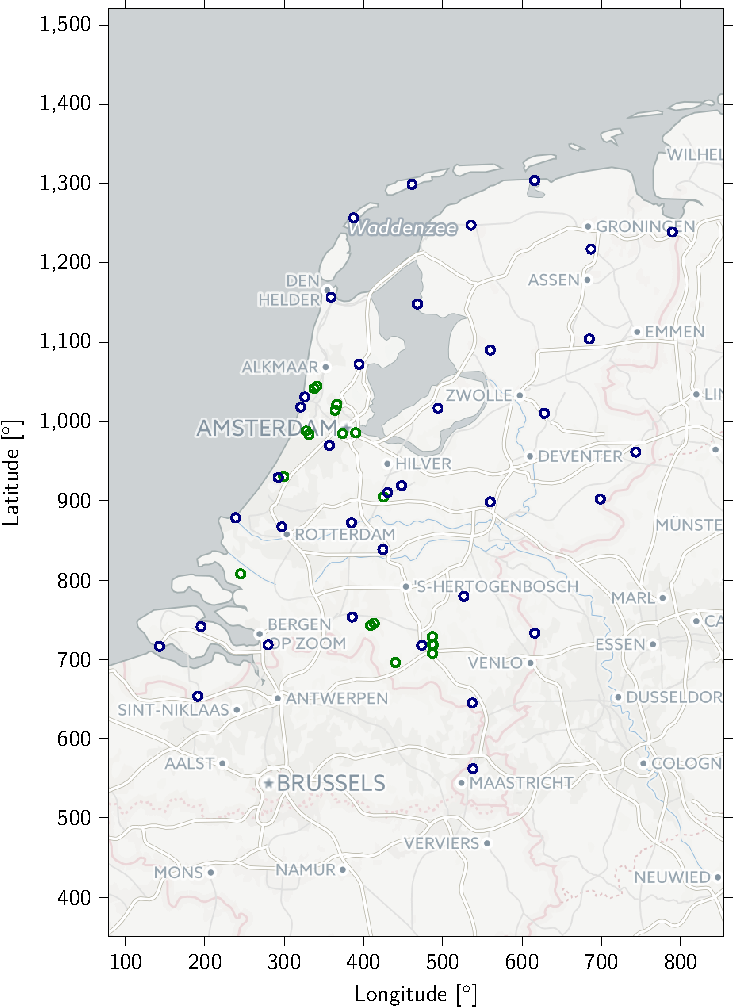
\includegraphics[width=.6\linewidth]{plots/detector/weather-map}
    \caption{This map shows the locations of all \hisparc (green) and \knmi (blue) weather stations.}
    \label{fig:weather-map}
\end{figure}

\begin{figure}
    \centering
    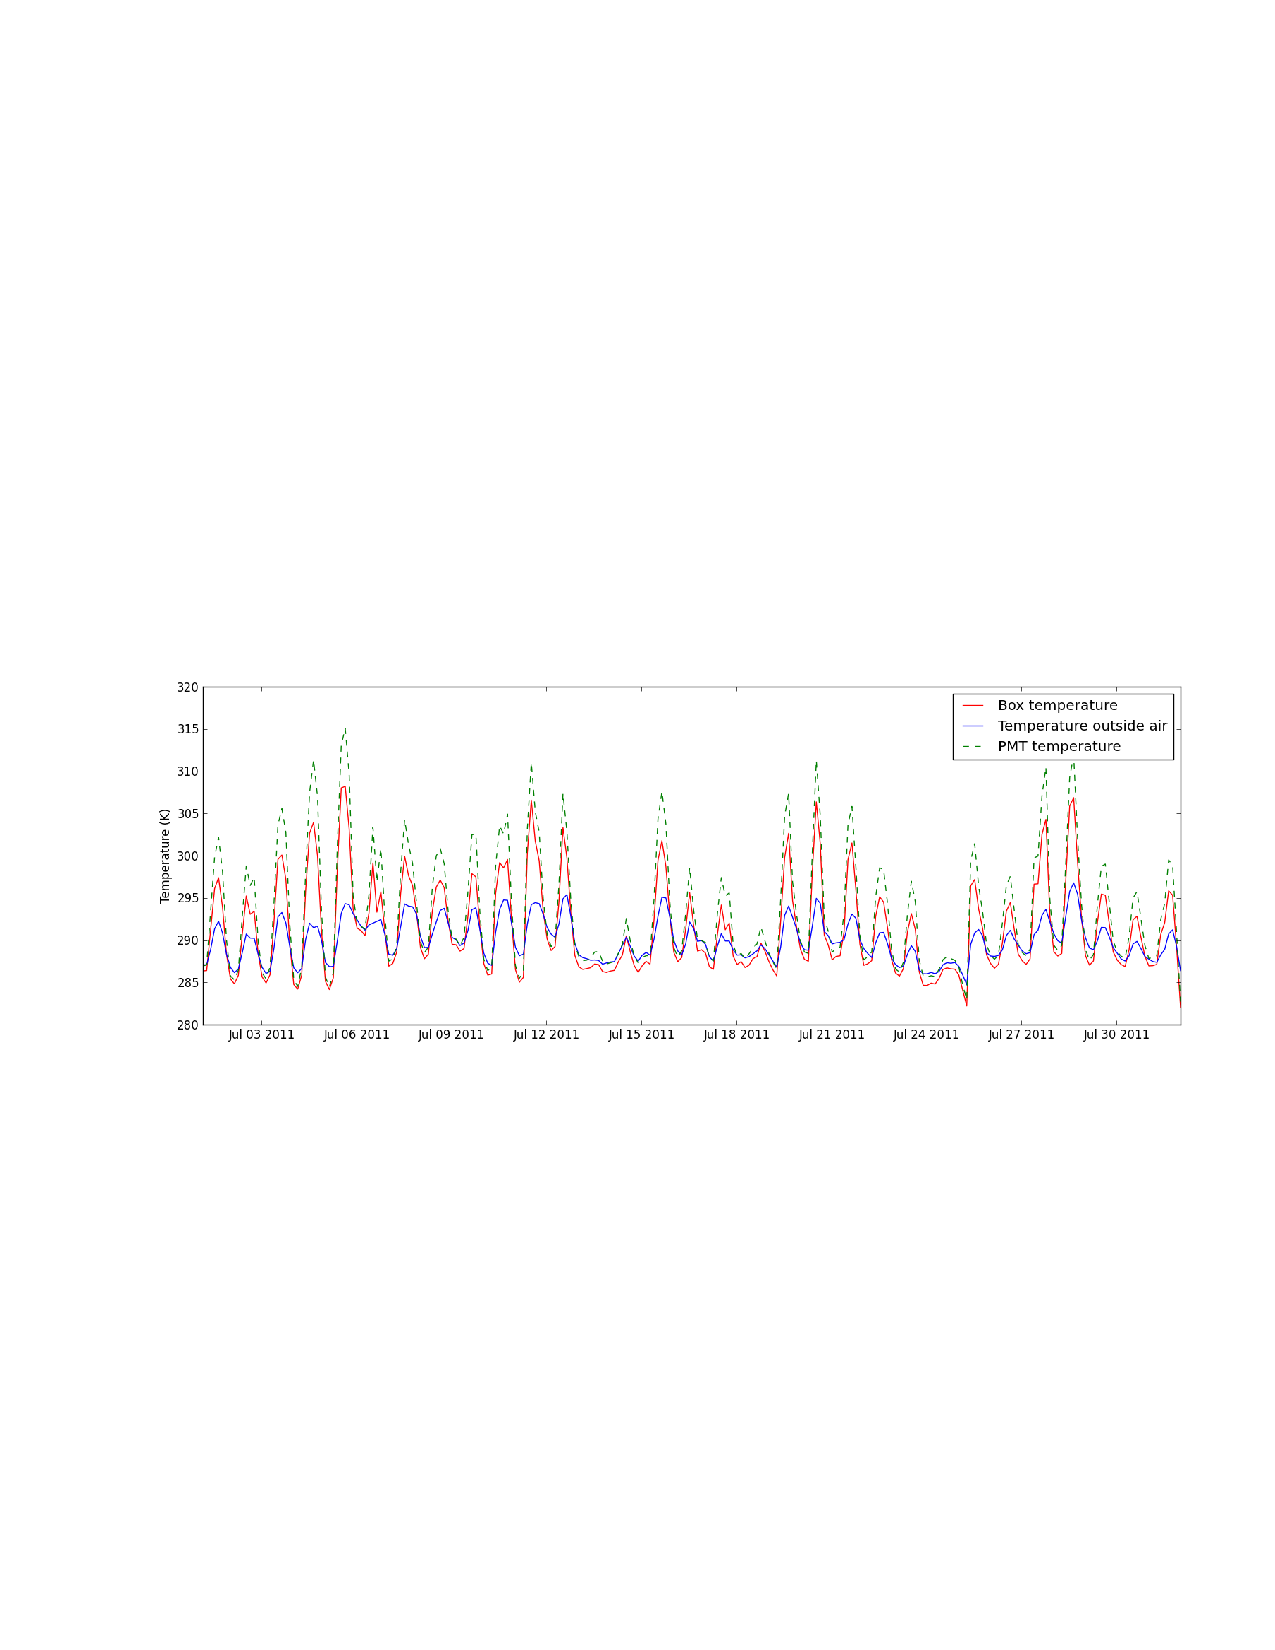
\includegraphics[width=\linewidth]{plots/detector/temperature_timeline}
    \caption{Measured temperatures over time from several different sensors. A temperature probe was placed inside a \hisparc detector skibox (blue). Another sensor was attached to the \pmt of the detector (green). The weather station connected to the \hisparc station also has a temperature sensor.}
    \label{fig:temperature_timeline}
\end{figure}

A day of data is enough to accurately determine the average MPV for that day. However, daily temperature fluctuation are large enough that when the days is broken into smaller pieces different values for the MPV are found \cite{bartels2012mpv}. In \cref{fig:mpv_temperature} the reconstructed MPV is set against the \pmt temperature. The spread around the fitted line is partially caused by the temperature gradient in the periods for which the MPV is determined. The correlation agrees reasonably with the specifications of the \pmt. The specification states the gain of the \pmt changes by \SI{0.5}{\percent\per\degreeCelsius}. It does not make clear wether the efficiency increases or decreases with changing temperature, nor at which temperature it is most efficient. From our measurements it seems the gain decreases with increasing temperature. The scintillator should be \SI{100}{\percent} effective upto \SI{20}{\degreeCelsius} above which it reduces with \SI{0.125}{\percent\per\degreeCelsius}. This is but a small contribution to the reduction of the MPV. The found gradient of \SI{-0.81}{\adc\per\degreeCelsius} in the range \SIrange{200}{170}{\adc} is \SI{0.44}{\percent\per\degreeCelsius}, in close agreement with the specification. (depends on what is used as reference..)

\begin{figure}
    \centering
    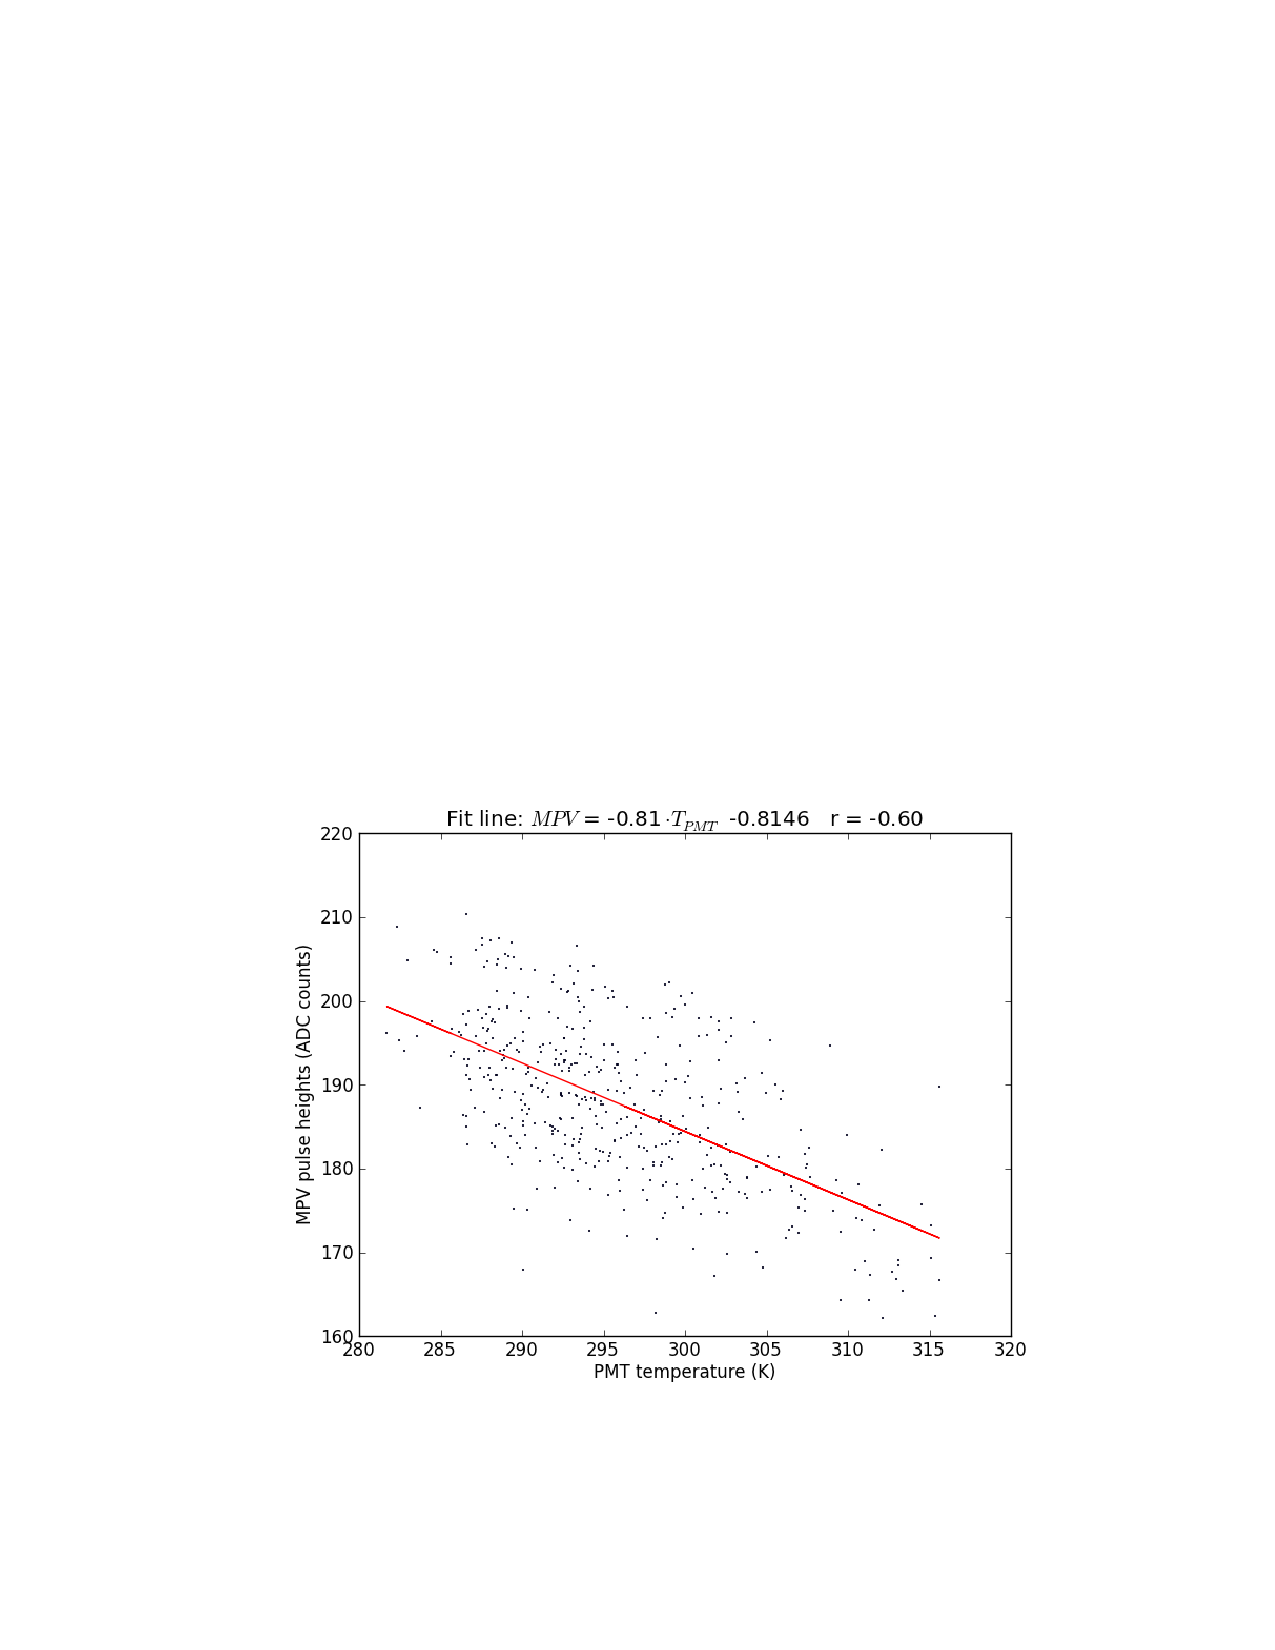
\includegraphics[width=.7\linewidth]{plots/detector/mpv_temperature}
    \caption{Here we can see the correlation between the measured temperature and the MPV of the pulse heights. The red line is a linear fit to get the slope of the correlation.}
    \label{fig:mpv_temperature}
\end{figure}

Weather station data is available to correct measurements for the change in efficiency. The correction can be done using the outside temperature and solar radiation. However, this is less accurate then when the exact PMT temperature is known. Solar radiation depends on cloud cover, which may be very different from location to location depending on wind speed. Moreover, some detectors may be in the shade for parts of the day, this may mean differences of \SI{20}{\degreeCelsius} between the expected and actual temperature.


\subsection{Air pressure}

The mean free path of shower particles is determined by the thickness of the air layer it passes through. If there are more particles to collide with the chance for interaction increases. An increase in air pressure reduces the mean free path. This means more interactions in a shower. \hisparc stations are far below Xmax so the extinction processes dominate. An increase in air pressure further reduces the number of particles reaching ground level and make detection less likely.

Air pressure data is available from the \hipsarc weather stations and also from KNMI data. In \cref{fig:rate_pressures} a correlation between the event rate in a station and the air pressure is shown.

\begin{figure}
    \centering
    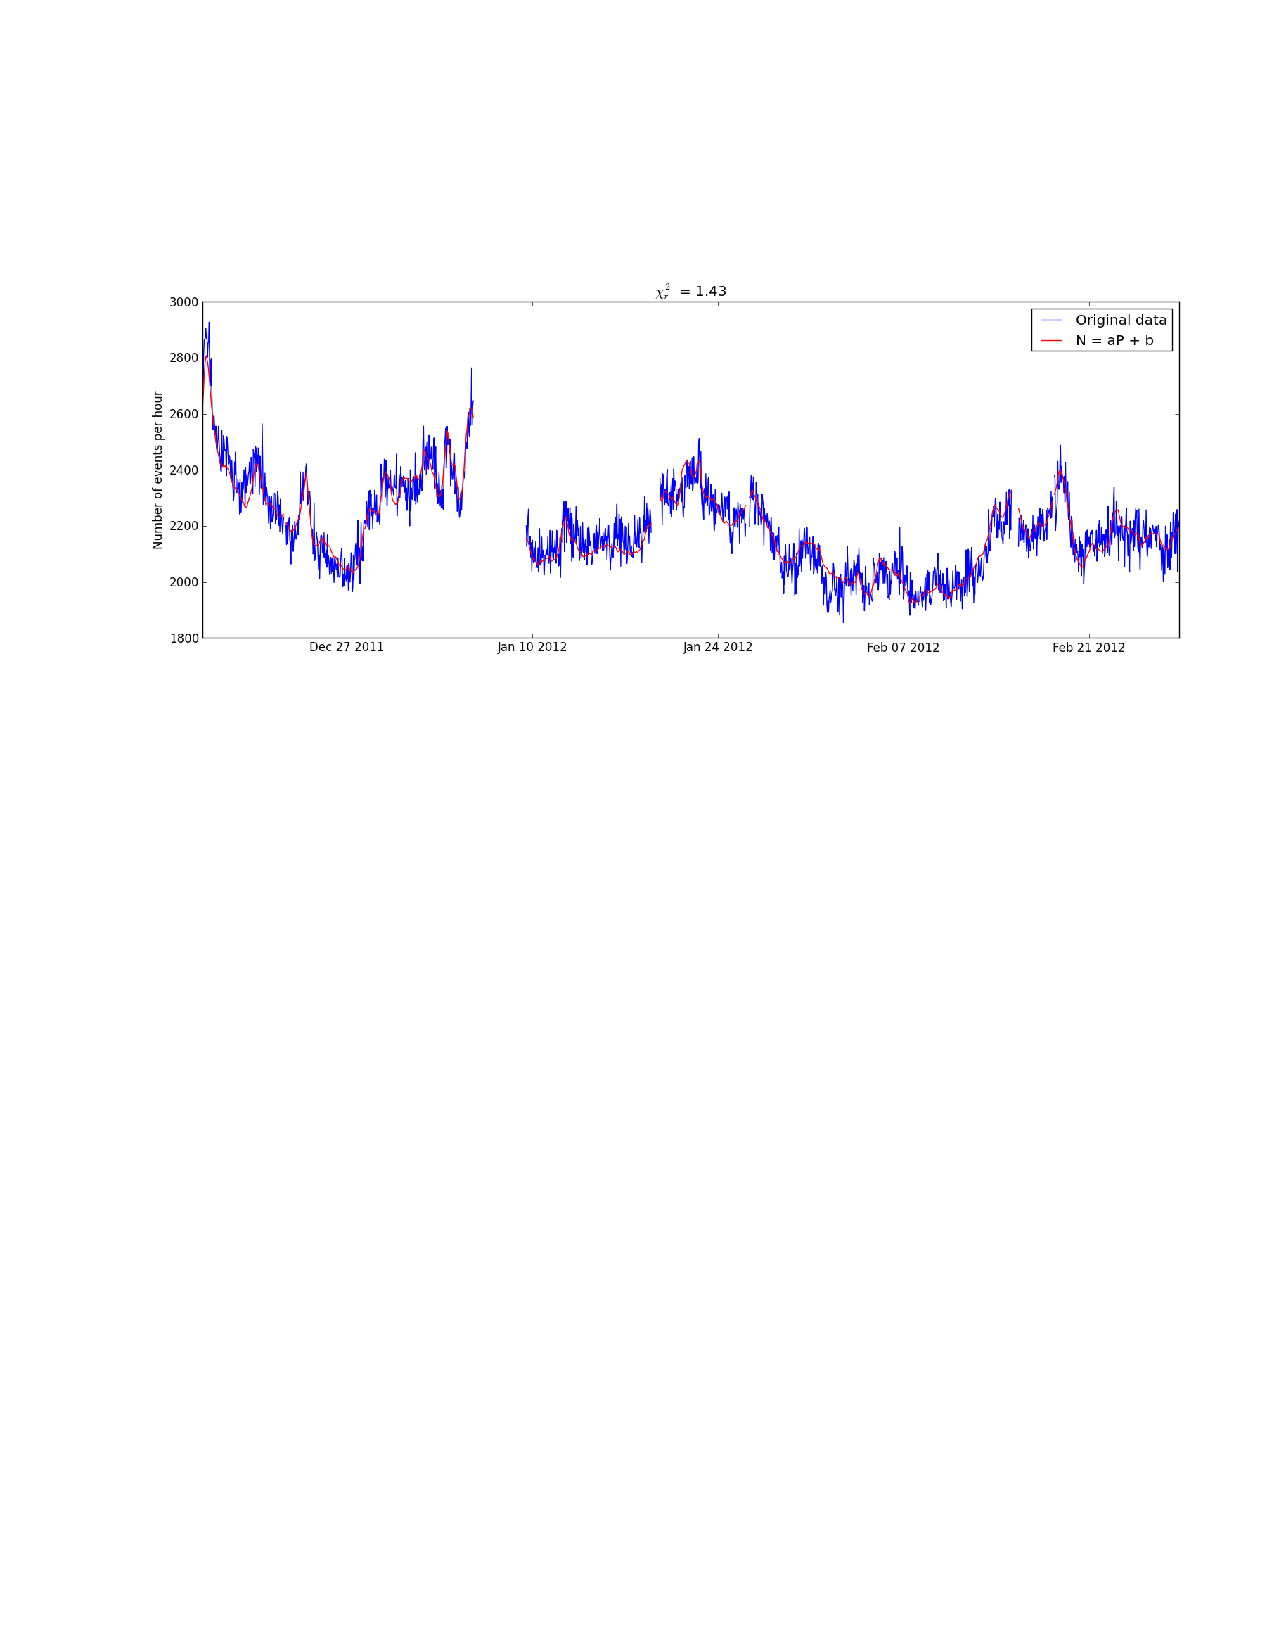
\includegraphics[width=.7\linewidth]{plots/detector/barometer}
    \caption{This shows the detected number of events fitted with a model that corrects the expectation using air pressure. A better match also considers temperature. Temperature can reduce or increase signal efficiency of a detector to make trigger less/more likely.}
    \label{fig:rate_pressures}
\end{figure}

The local air pressure is to be taken into account when determining the shower energy. The relation between shower size and shower energy depends on air pressure. Air pressure does not affect the signal generated by \mips.

[Describe how much uncertainty this adds to density reconstruction.]


\section{Durability}
\label{sec:detector-durability}

Light leaks, often directly evident after construction, some develop over time. Can be discovered in multiple ways (event rate/number of peaks). Often easy to fix by applying extra foil and tape.

The connection between the scintillator and lightguide (glue) sometimes breaks, the detector may still works but with different efficiency. As long as the detector is not moved and properly supported it can continue to operate indefinitely. Repairing the detector takes as much time as the initial construction. The glued edges needs to be sanded again.

In the small time period shown in \cref{fig:temperature_timeline} temperatures above \SI{42}{\degreeCelsius} are seen. The specifications of the \pmt state its maximum operational temperature as \SI{60}{\degreeCelsius}. Such high temperatures likely occur occasionally. However, this does not seem to be an issue.

A batch of \pmts has been encountered where the failure rate was very high, around 30 \pmts failed. This is quite a significant number since we have approximately 300 \pmts in use. The power supplies of these \pmts failed. The actual vacuum tubes were still working fine. The costs to have the power supply replaced by the manufacturer were excessive, almost equal to a new \pmt. This was one of the motivations to manufacture \pmt bases. Replacing \pmts is an easy process, this can be performed without moving the detector.

The power supplies provides by the company that assembled the HiSPARC electronics were a bad batch. They all fail within a couple months of use. These have been replaced by a different type of power supply of which no failures have been observed. Not all electronics were deployed at once, so preemptive replacements have been done for those deployed later.

On some occasions power interruptions can cause down time for a station.  There are cases where supplies were disconnected by cleaning crews or students that wanted to use the power socket for their own devices. Some schools disable their power grid during vacation time, in order to save power. Usually the station resumes operation after the vacation when the power is restored.

Despite these possible problems most detectors perform perfectly for many years, and problems can be addressed easily, as was the goal.
